\documentclass[tikz,border=6pt]{standalone}
\usepackage{tikz}
\begin{document}
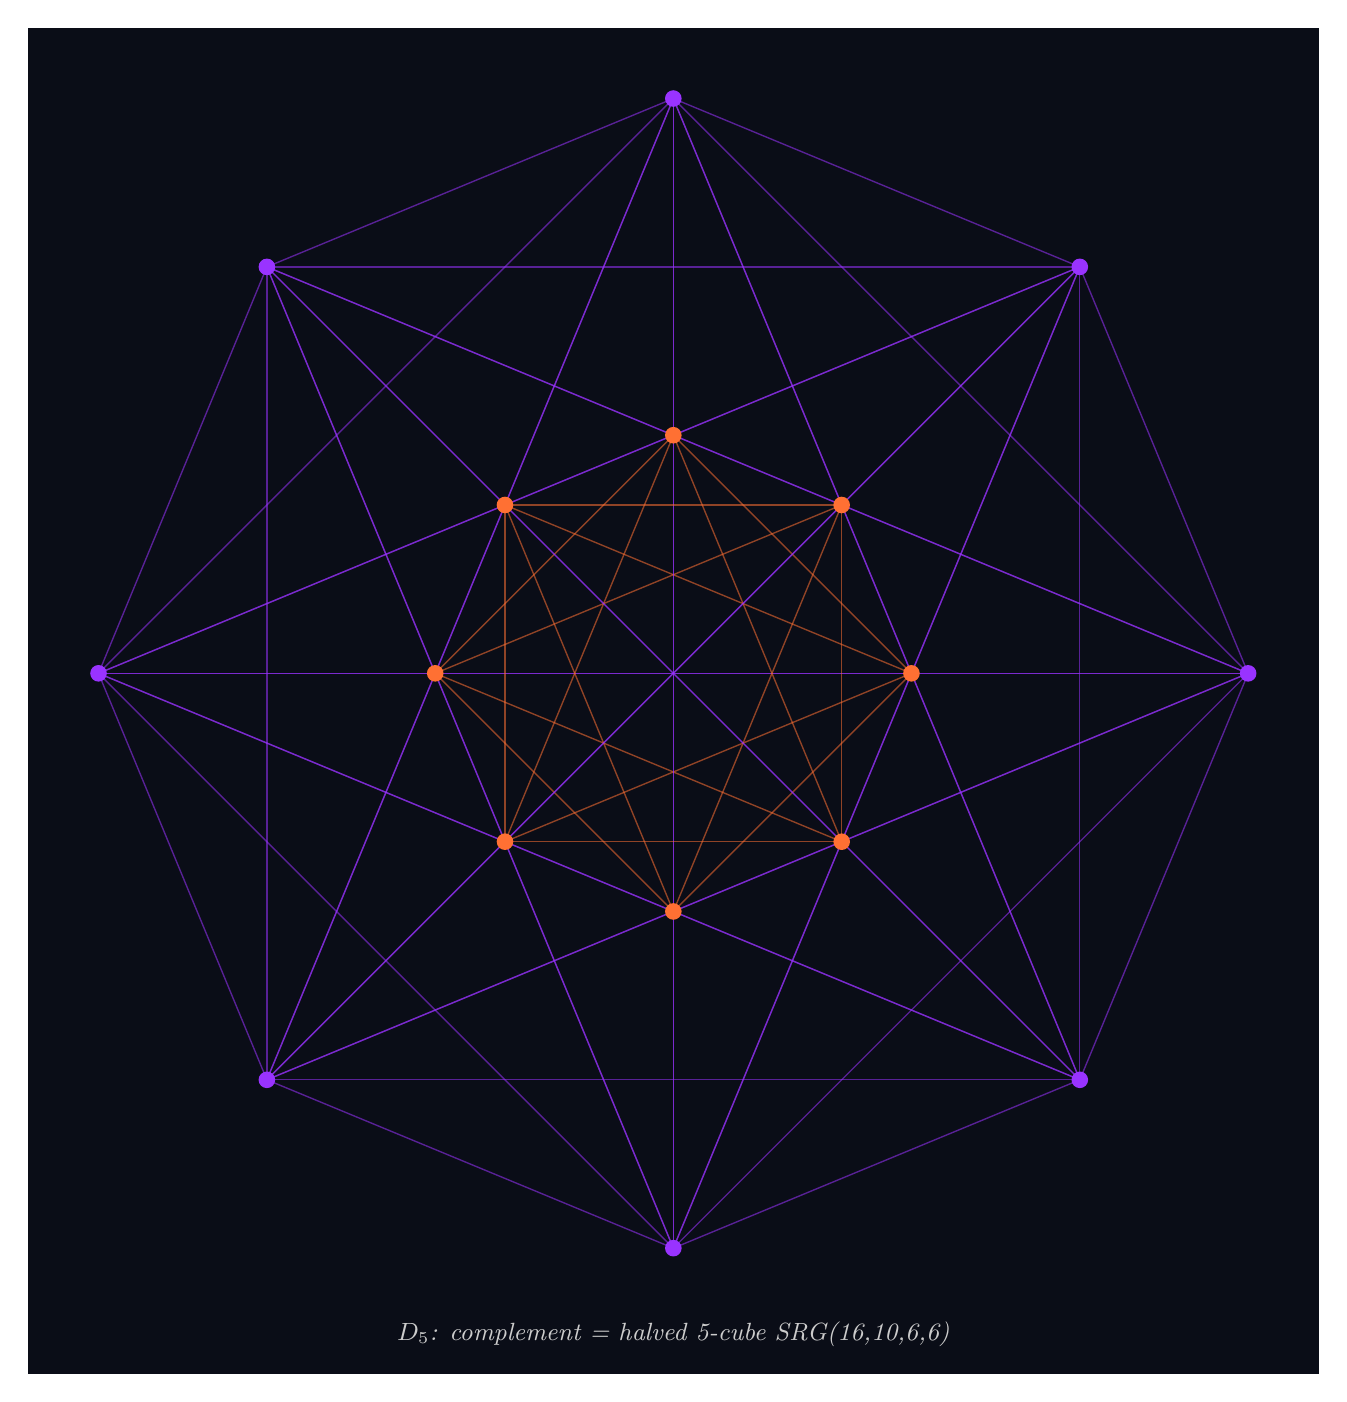
\begin{tikzpicture}
\definecolor{ring0}{rgb}{1.000,0.440,0.200}
\definecolor{ring1}{rgb}{0.600,0.200,1.000}
\definecolor{bg}{rgb}{0.04,0.05,0.09}
\fill[bg] (-8.2,-8.9) rectangle (8.2,8.2);
\draw[ring1,line width=0.5pt,opacity=0.55] (-7.300,0.000)--(-3.024,0.000);
\draw[ring1,line width=0.5pt,opacity=0.55] (-7.300,0.000)--(3.024,-0.000);
\draw[ring1,line width=0.5pt,opacity=0.55] (-7.300,0.000)--(-0.000,-3.024);
\draw[ring1,line width=0.5pt,opacity=0.55] (-7.300,0.000)--(0.000,3.024);
\draw[ring1,line width=0.5pt,opacity=0.55] (-7.300,0.000)--(-0.000,-7.300);
\draw[ring1,line width=0.5pt,opacity=0.55] (-7.300,0.000)--(0.000,7.300);
\draw[ring1,line width=0.5pt,opacity=0.55] (-7.300,0.000)--(-5.162,-5.162);
\draw[ring1,line width=0.5pt,opacity=0.55] (-7.300,0.000)--(-5.162,5.162);
\draw[ring1,line width=0.5pt,opacity=0.55] (-7.300,0.000)--(-2.138,2.138);
\draw[ring1,line width=0.5pt,opacity=0.55] (-7.300,0.000)--(-2.138,-2.138);
\draw[ring1,line width=0.5pt,opacity=0.55] (7.300,-0.000)--(-3.024,0.000);
\draw[ring1,line width=0.5pt,opacity=0.55] (7.300,-0.000)--(3.024,-0.000);
\draw[ring1,line width=0.5pt,opacity=0.55] (7.300,-0.000)--(-0.000,-3.024);
\draw[ring1,line width=0.5pt,opacity=0.55] (7.300,-0.000)--(0.000,3.024);
\draw[ring1,line width=0.5pt,opacity=0.55] (7.300,-0.000)--(-0.000,-7.300);
\draw[ring1,line width=0.5pt,opacity=0.55] (7.300,-0.000)--(0.000,7.300);
\draw[ring1,line width=0.5pt,opacity=0.55] (7.300,-0.000)--(2.138,2.138);
\draw[ring1,line width=0.5pt,opacity=0.55] (7.300,-0.000)--(2.138,-2.138);
\draw[ring1,line width=0.5pt,opacity=0.55] (7.300,-0.000)--(5.162,-5.162);
\draw[ring1,line width=0.5pt,opacity=0.55] (7.300,-0.000)--(5.162,5.162);
\draw[ring0,line width=0.5pt,opacity=0.55] (-3.024,0.000)--(-0.000,-3.024);
\draw[ring0,line width=0.5pt,opacity=0.55] (-3.024,0.000)--(0.000,3.024);
\draw[ring1,line width=0.5pt,opacity=0.55] (-3.024,0.000)--(-0.000,-7.300);
\draw[ring1,line width=0.5pt,opacity=0.55] (-3.024,0.000)--(0.000,7.300);
\draw[ring1,line width=0.5pt,opacity=0.55] (-3.024,0.000)--(-5.162,-5.162);
\draw[ring1,line width=0.5pt,opacity=0.55] (-3.024,0.000)--(-5.162,5.162);
\draw[ring0,line width=0.5pt,opacity=0.55] (-3.024,0.000)--(2.138,2.138);
\draw[ring0,line width=0.5pt,opacity=0.55] (-3.024,0.000)--(2.138,-2.138);
\draw[ring0,line width=0.5pt,opacity=0.55] (3.024,-0.000)--(-0.000,-3.024);
\draw[ring0,line width=0.5pt,opacity=0.55] (3.024,-0.000)--(0.000,3.024);
\draw[ring1,line width=0.5pt,opacity=0.55] (3.024,-0.000)--(-0.000,-7.300);
\draw[ring1,line width=0.5pt,opacity=0.55] (3.024,-0.000)--(0.000,7.300);
\draw[ring0,line width=0.5pt,opacity=0.55] (3.024,-0.000)--(-2.138,2.138);
\draw[ring0,line width=0.5pt,opacity=0.55] (3.024,-0.000)--(-2.138,-2.138);
\draw[ring1,line width=0.5pt,opacity=0.55] (3.024,-0.000)--(5.162,-5.162);
\draw[ring1,line width=0.5pt,opacity=0.55] (3.024,-0.000)--(5.162,5.162);
\draw[ring1,line width=0.5pt,opacity=0.55] (-0.000,-3.024)--(-0.000,-7.300);
\draw[ring1,line width=0.5pt,opacity=0.55] (-0.000,-3.024)--(0.000,7.300);
\draw[ring1,line width=0.5pt,opacity=0.55] (-0.000,-3.024)--(-5.162,-5.162);
\draw[ring0,line width=0.5pt,opacity=0.55] (-0.000,-3.024)--(-2.138,2.138);
\draw[ring0,line width=0.5pt,opacity=0.55] (-0.000,-3.024)--(2.138,2.138);
\draw[ring1,line width=0.5pt,opacity=0.55] (-0.000,-3.024)--(5.162,-5.162);
\draw[ring1,line width=0.5pt,opacity=0.55] (0.000,3.024)--(-0.000,-7.300);
\draw[ring1,line width=0.5pt,opacity=0.55] (0.000,3.024)--(0.000,7.300);
\draw[ring1,line width=0.5pt,opacity=0.55] (0.000,3.024)--(-5.162,5.162);
\draw[ring0,line width=0.5pt,opacity=0.55] (0.000,3.024)--(-2.138,-2.138);
\draw[ring0,line width=0.5pt,opacity=0.55] (0.000,3.024)--(2.138,-2.138);
\draw[ring1,line width=0.5pt,opacity=0.55] (0.000,3.024)--(5.162,5.162);
\draw[ring1,line width=0.5pt,opacity=0.55] (-0.000,-7.300)--(-5.162,-5.162);
\draw[ring1,line width=0.5pt,opacity=0.55] (-0.000,-7.300)--(-2.138,-2.138);
\draw[ring1,line width=0.5pt,opacity=0.55] (-0.000,-7.300)--(2.138,-2.138);
\draw[ring1,line width=0.5pt,opacity=0.55] (-0.000,-7.300)--(5.162,-5.162);
\draw[ring1,line width=0.5pt,opacity=0.55] (0.000,7.300)--(-5.162,5.162);
\draw[ring1,line width=0.5pt,opacity=0.55] (0.000,7.300)--(-2.138,2.138);
\draw[ring1,line width=0.5pt,opacity=0.55] (0.000,7.300)--(2.138,2.138);
\draw[ring1,line width=0.5pt,opacity=0.55] (0.000,7.300)--(5.162,5.162);
\draw[ring1,line width=0.5pt,opacity=0.55] (-5.162,-5.162)--(-5.162,5.162);
\draw[ring1,line width=0.5pt,opacity=0.55] (-5.162,-5.162)--(-2.138,2.138);
\draw[ring1,line width=0.5pt,opacity=0.55] (-5.162,-5.162)--(-2.138,-2.138);
\draw[ring1,line width=0.5pt,opacity=0.55] (-5.162,-5.162)--(2.138,2.138);
\draw[ring1,line width=0.5pt,opacity=0.55] (-5.162,-5.162)--(2.138,-2.138);
\draw[ring1,line width=0.5pt,opacity=0.55] (-5.162,-5.162)--(5.162,-5.162);
\draw[ring1,line width=0.5pt,opacity=0.55] (-5.162,5.162)--(-2.138,2.138);
\draw[ring1,line width=0.5pt,opacity=0.55] (-5.162,5.162)--(-2.138,-2.138);
\draw[ring1,line width=0.5pt,opacity=0.55] (-5.162,5.162)--(2.138,2.138);
\draw[ring1,line width=0.5pt,opacity=0.55] (-5.162,5.162)--(2.138,-2.138);
\draw[ring1,line width=0.5pt,opacity=0.55] (-5.162,5.162)--(5.162,5.162);
\draw[ring0,line width=0.5pt,opacity=0.55] (-2.138,2.138)--(-2.138,-2.138);
\draw[ring0,line width=0.5pt,opacity=0.55] (-2.138,2.138)--(2.138,2.138);
\draw[ring1,line width=0.5pt,opacity=0.55] (-2.138,2.138)--(5.162,-5.162);
\draw[ring1,line width=0.5pt,opacity=0.55] (-2.138,2.138)--(5.162,5.162);
\draw[ring0,line width=0.5pt,opacity=0.55] (-2.138,-2.138)--(2.138,-2.138);
\draw[ring1,line width=0.5pt,opacity=0.55] (-2.138,-2.138)--(5.162,-5.162);
\draw[ring1,line width=0.5pt,opacity=0.55] (-2.138,-2.138)--(5.162,5.162);
\draw[ring0,line width=0.5pt,opacity=0.55] (2.138,2.138)--(2.138,-2.138);
\draw[ring1,line width=0.5pt,opacity=0.55] (2.138,2.138)--(5.162,-5.162);
\draw[ring1,line width=0.5pt,opacity=0.55] (2.138,2.138)--(5.162,5.162);
\draw[ring1,line width=0.5pt,opacity=0.55] (2.138,-2.138)--(5.162,-5.162);
\draw[ring1,line width=0.5pt,opacity=0.55] (2.138,-2.138)--(5.162,5.162);
\draw[ring1,line width=0.5pt,opacity=0.55] (5.162,-5.162)--(5.162,5.162);
\fill[ring1] (-7.300,0.000) circle (3.0pt);
\fill[ring1] (7.300,-0.000) circle (3.0pt);
\fill[ring0] (-3.024,0.000) circle (3.0pt);
\fill[ring0] (3.024,-0.000) circle (3.0pt);
\fill[ring0] (-0.000,-3.024) circle (3.0pt);
\fill[ring0] (0.000,3.024) circle (3.0pt);
\fill[ring1] (-0.000,-7.300) circle (3.0pt);
\fill[ring1] (0.000,7.300) circle (3.0pt);
\fill[ring1] (-5.162,-5.162) circle (3.0pt);
\fill[ring1] (-5.162,5.162) circle (3.0pt);
\fill[ring0] (-2.138,2.138) circle (3.0pt);
\fill[ring0] (-2.138,-2.138) circle (3.0pt);
\fill[ring0] (2.138,2.138) circle (3.0pt);
\fill[ring0] (2.138,-2.138) circle (3.0pt);
\fill[ring1] (5.162,-5.162) circle (3.0pt);
\fill[ring1] (5.162,5.162) circle (3.0pt);
\node[white!80!black,font=\small\itshape] at (0,-8.4) {$D_5$: complement = halved 5-cube SRG(16,10,6,6)};
\end{tikzpicture}
\end{document}